This subsection is used when we have to save or retrieve data from the database. When user tries to login, register, add self, add item or search we have to use database. When somebody wants to register for the app, he provides all the information then these information is taken by the DB controller and saved in organized manner. same process occurs for all the other activities like adding self, adding item or login.

\subsection{Layer Hardware}
N/A

\subsection{Layer Operating System}
IOS/Android

\subsection{Layer Software Dependencies}
Firebase, Internal Memory,


\subsection{DB Controller}
This is a type of main controller of the Database system. All the data that needs to be stored in database is first handled by this layer and later stored in the database. When any of the other layer send data to the database layer, first database layer takes the information and figures out what type of data is provided and what to do with the given data.

\begin{figure}[h!]
	\centering
 	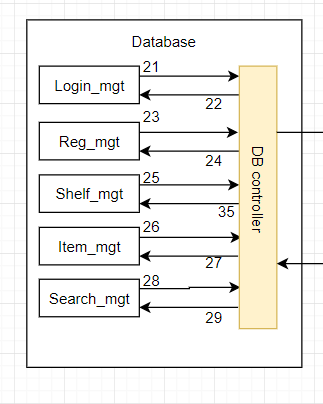
\includegraphics[width=0.60\textwidth]{images/dbcontroller}
 \caption{DB Controller description diagram}
\end{figure}

\subsubsection{DB Controller Hardware}
Internal Memory

\subsubsection{DB Controller Operating System}
iOS/Android

\subsubsection{DB Controller Software Dependencies}
\begin{rand}"dependencies":\\ {
    "expo": "34.0.1",\\    \
    "expo-permissions": "6.0.0",\\
    "firebase": "6.6.0",\\
    "react": "16.8.3",\\
    "react-native": "https://github.com/expo/react-native/archive/sdk-34.0.0.tar.gz",\\
    "react-navigation-stack": "1.5.1",\\
\end{rand}

\subsubsection{DB Controller Programming Languages}
JavaScript

\subsubsection{DB Controller Data Structures}
JSON, Array, Objects

\subsubsection{DB Controller Data Processing}
Depending upon the data provided by the user, data will be sent to the subsystems of database ie. login\_mgt, Reg\_mgt, Shelf\_mgt, Item\_mgt, Search\_mgt.
According to the query of the user database willthe subsystems ie. login\_mgt, Reg\_mgt, Shelf\_mgt, Item\_mgt, Search\_mgt and help user in validation of user and fetching of data.


\subsection{Login Mgt}
This subsection of database just deals with the login information. User first registers for the account in the mobile application. Then when he wants to use the app he will provide the user name and password for the app. Then the login management layer handles all the data. It checks if the user name and password provided by the user exists in database or not. It should allow user to login if the combination of user name and password exists else it should deny user from using the application itself.

\begin{figure}[h!]
	\centering
 	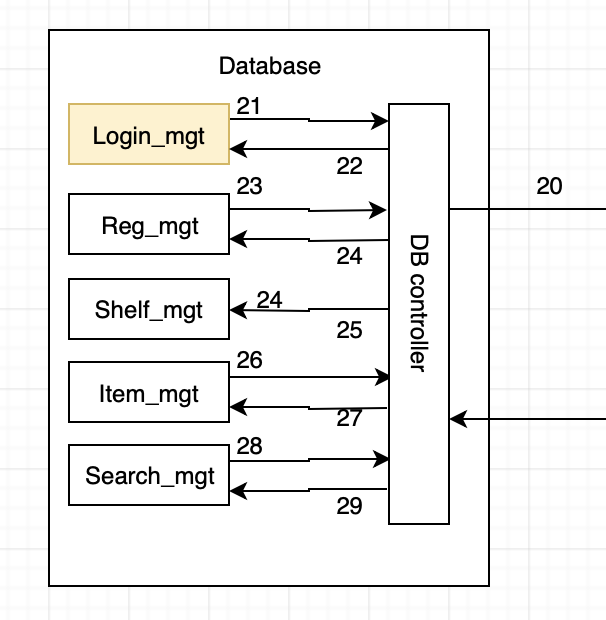
\includegraphics[width=0.60\textwidth]{images/loginmgt}
 \caption{Login mgt description diagram}
\end{figure}

\subsubsection{Login Mgt Hardware}
Internal Memory

\subsubsection{Login Mgt Operating System}
iOS/Android

\subsubsection{Login Mgt Software Dependencies}
\begin{rand}"dependencies":\\ {
    "expo": "34.0.1",\\
    "expo-permissions": "6.0.0",\\
    "firebase": "6.6.0",\\
    "react": "16.8.3",\\ "react-native-gesture-handler": "1.4.1",\\
    "react-navigation-stack": "1.5.1",\\
    "reinput": "3.7.1"]\\
\end{rand}

\subsubsection{Login Mgt Programming Languages}
JavaScript

\subsubsection{Login Mgt Data Structures}
JSON, Array, Objects

\subsubsection{Login Mgt Data Processing}
Depending upon the data provided by the user, data will be sent to the subsystem ie. login\_mgt. Login\_mgt will then validate the user if the username and password is correct. 
This will return a boolean result if the user is authorized or not.



\subsection{Register Mgt}
This subsection of the database deals with registration data like first name, last name, DOB,etc. When user provides the information it is validated for SQL injection and passed into the register management. Then the data is stored in database in organized manner by the register management subsystem.

\begin{figure}[h!]
	\centering
 	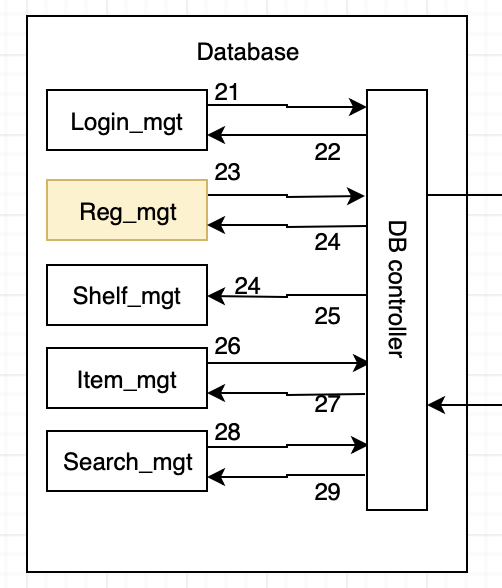
\includegraphics[width=0.60\textwidth]{images/regmgt}
 \caption{Register mgt description diagram}
\end{figure}


\subsubsection{Register Mgt Hardware}
Internal Memory

\subsubsection{Register Mgt Operating System}
iOS/Android

\subsubsection{Register Mgt Software Dependencies}
\begin{rand}"dependencies":\\ {
    "expo": "34.0.1",\\
    "expo-permissions": "6.0.0",\\
    "firebase": "6.6.0",\\
    "react": "16.8.3",\\ "react-native-gesture-handler": "1.4.1",\\
    "react-navigation-stack": "1.5.1",\\
    "reinput": "3.7.1"]\\
\end{rand}

\subsubsection{Register Mgt Programming Languages}
JavaScript

\subsubsection{Register Mgt Data Structures}
JSON, Array, Objects

\subsubsection{Register Mgt Data Processing}
Depending upon the data provided by the user, data will be sent to the subsystem ie. Register\_mgt. Register\_mgt will then validate the user if the username and password is correct. 
This will return a boolean result if the user is authorized or not.

\subsection{Item mgt}
This subsystem of the database is used whenever user wants to add or remove item from the database. When user provides the data for adding or removing the item, then the DB controller takes the input at first and then passes it to the item Mgmt. Then the layer takes the input value and make necessary change ie. add or remove the item accordingly.

\begin{figure}[h!]
	\centering
 	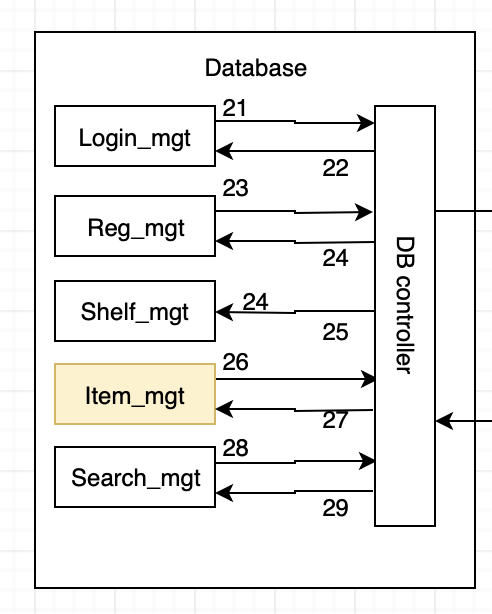
\includegraphics[width=0.60\textwidth]{images/itemmgt}
 \caption{Item mgt description diagram}
\end{figure}

\subsubsection{Item Mgt Hardware}
Internal Memory

\subsubsection{Item Mgt Operating System}
IOS/Android


























































\subsubsection{Item Mgt Software Dependencies}
\begin{rand}"dependencies":\\ {
    "expo": "34.0.1",\\
    "expo-permissions": "6.0.0",\\
    "firebase": "6.6.0",\\
    "react": "16.8.3",\\ "react-native-gesture-handler": "1.4.1",\\
    "react-navigation-stack": "1.5.1",\\
    "reinput": "3.7.1"]\\
\end{rand}

\subsubsection{Item Mgt Programming Languages}
JavaScript

\subsubsection{Item Mgt Data Structures}
JSON, Array, Objects

\subsubsection{Item Mgt Data Processing}
Depending upon the data provided by the user, data will stored in the logged in user's database.

\subsection{Search mgt}
This Sub System deals with taking the item description from user and it searches for the item. Variety of options are provided for searching the item. User can use the camera in the cellphone to scan the QR generated for the specific item or users will also be able to search the item by their names.

\begin{figure}[h!]
	\centering
 	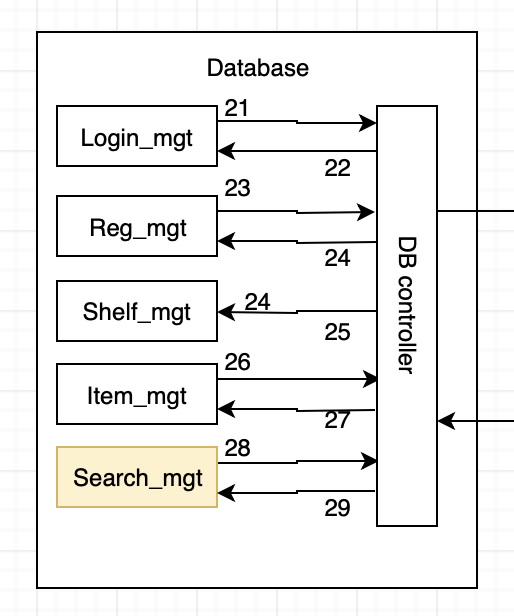
\includegraphics[width=0.60\textwidth]{images/searchmgt}
 \caption{Search mgt description diagram}
\end{figure}

\subsubsection{Search Mgt Hardware}
Phone display

\subsubsection{Search Mgt Operating System}
IOS/Android

\subsubsection{Search Mgt Software Dependencies}
\begin{rand}"dependencies":\\ {
    "expo": "34.0.1",\\
    "expo-permissions": "6.0.0",\\
    "firebase": "6.6.0",\\
    "react": "16.8.3",\\ "react-native-gesture-handler": "1.4.1",\\
    "react-navigation-stack": "1.5.1",\\
    "reinput": "3.7.1"]\\
\end{rand}

\subsubsection{Search Mgt Programming Languages}
JavaScript

\subsubsection{Search Mgt Data Structures}
 Array, Objects, Union

\subsubsection{Search Mgt Data Processing}
Depending upon the data provided by the user, data will be retrieved from logged in user's database.

